\documentclass[multi=tikzpicture,border=8pt]{standalone}
\usepackage{fontspec}
\usepackage{amssymb}
\usepackage{xcolor}
\usepackage{tikz}
\usetikzlibrary{arrows.meta,calc,positioning,shadows.blur}

\setmainfont{Latin Modern Sans}

\definecolor{substrate}{HTML}{1F4E79}
\definecolor{matter}{HTML}{2E7D32}
\definecolor{gauge}{HTML}{00838F}
\definecolor{cosmo}{HTML}{EF6C00}
\definecolor{dark}{HTML}{6A1B9A}
\definecolor{gravity}{HTML}{B71C1C}
\definecolor{relativity}{HTML}{AD1457}
\definecolor{method}{HTML}{616161}
\definecolor{derivedfill}{HTML}{E8F2FF}
\definecolor{condfill}{HTML}{FFF3D6}
\definecolor{openfill}{HTML}{F2E7FA}
\definecolor{importfill}{HTML}{EEEEEE}
\definecolor{retiredfill}{HTML}{FBE9E7}

\tikzset{
  route/.style={line width=4.0pt, line cap=round, line join=round},
  soft/.style={line width=1.4pt, line cap=round, line join=round},
  edge/.style={soft, -{Latex[length=2.0mm]}, draw=method!72},
  station/.style={
    rounded corners=3pt,
    draw=black!45,
    line width=0.45pt,
    fill=white,
    align=center,
    font=\scriptsize,
    inner xsep=3pt,
    inner ysep=2.5pt,
    text width=2.35cm
  },
  hub/.style={
    rounded corners=4pt,
    draw=black!55,
    line width=0.55pt,
    fill=white,
    blur shadow={shadow blur steps=4, shadow xshift=0.5pt, shadow yshift=-0.5pt, shadow opacity=16},
    align=center,
    font=\scriptsize\bfseries,
    inner xsep=4pt,
    inner ysep=3pt,
    text width=2.55cm
  },
  derived/.style={fill=derivedfill, draw=substrate!70},
  conditional/.style={fill=condfill, draw=cosmo!85},
  open/.style={fill=openfill, draw=dark!80, dashed},
  imported/.style={fill=importfill, draw=method!70},
  retired/.style={fill=retiredfill, draw=red!70, densely dashed},
  label/.style={font=\tiny, text=black!67, align=center},
  routeLabel/.style={font=\scriptsize\bfseries, align=left},
  note/.style={font=\tiny, text=black!62, align=left},
  capsule/.style={font=\tiny, rounded corners=2pt, draw=black!20, fill=white, inner xsep=3pt, inner ysep=1.5pt, align=center}
}

\newcommand{\pageframe}[3]{%
  \path[use as bounding box] (0,0) rectangle (20,11.5);
  \fill[white] (0,0) rectangle (20,11.5);
  \node[font=\Large\bfseries, anchor=west] at (0.25,10.95) {#1};
  \node[font=\small, text=black!62, anchor=west] at (0.25,10.55) {#2};
  \node[font=\tiny, text=black!52, anchor=east] at (19.75,0.35) {#3};
}

\newcommand{\legendblock}{%
  \node[anchor=north west, draw=black!18, rounded corners=3pt, fill=white, inner sep=4pt, font=\tiny, align=left] at (0.25,2.05) {
    \textbf{Status}\\[2pt]
    \tikz{\node[station, derived, minimum width=0.45cm, text width=0.22cm]{};} derived / script-backed\\
    \tikz{\node[station, conditional, minimum width=0.45cm, text width=0.22cm]{};} conditional closure\\
    \tikz{\node[station, open, minimum width=0.45cm, text width=0.22cm]{};} open blocker\\
    \tikz{\node[station, imported, minimum width=0.45cm, text width=0.22cm]{};} imported theorem\\
    grey arrows: proof dependency
  };
}

\begin{document}

% ---------------------------------------------------------------------------
% Page 1: overview.
% ---------------------------------------------------------------------------
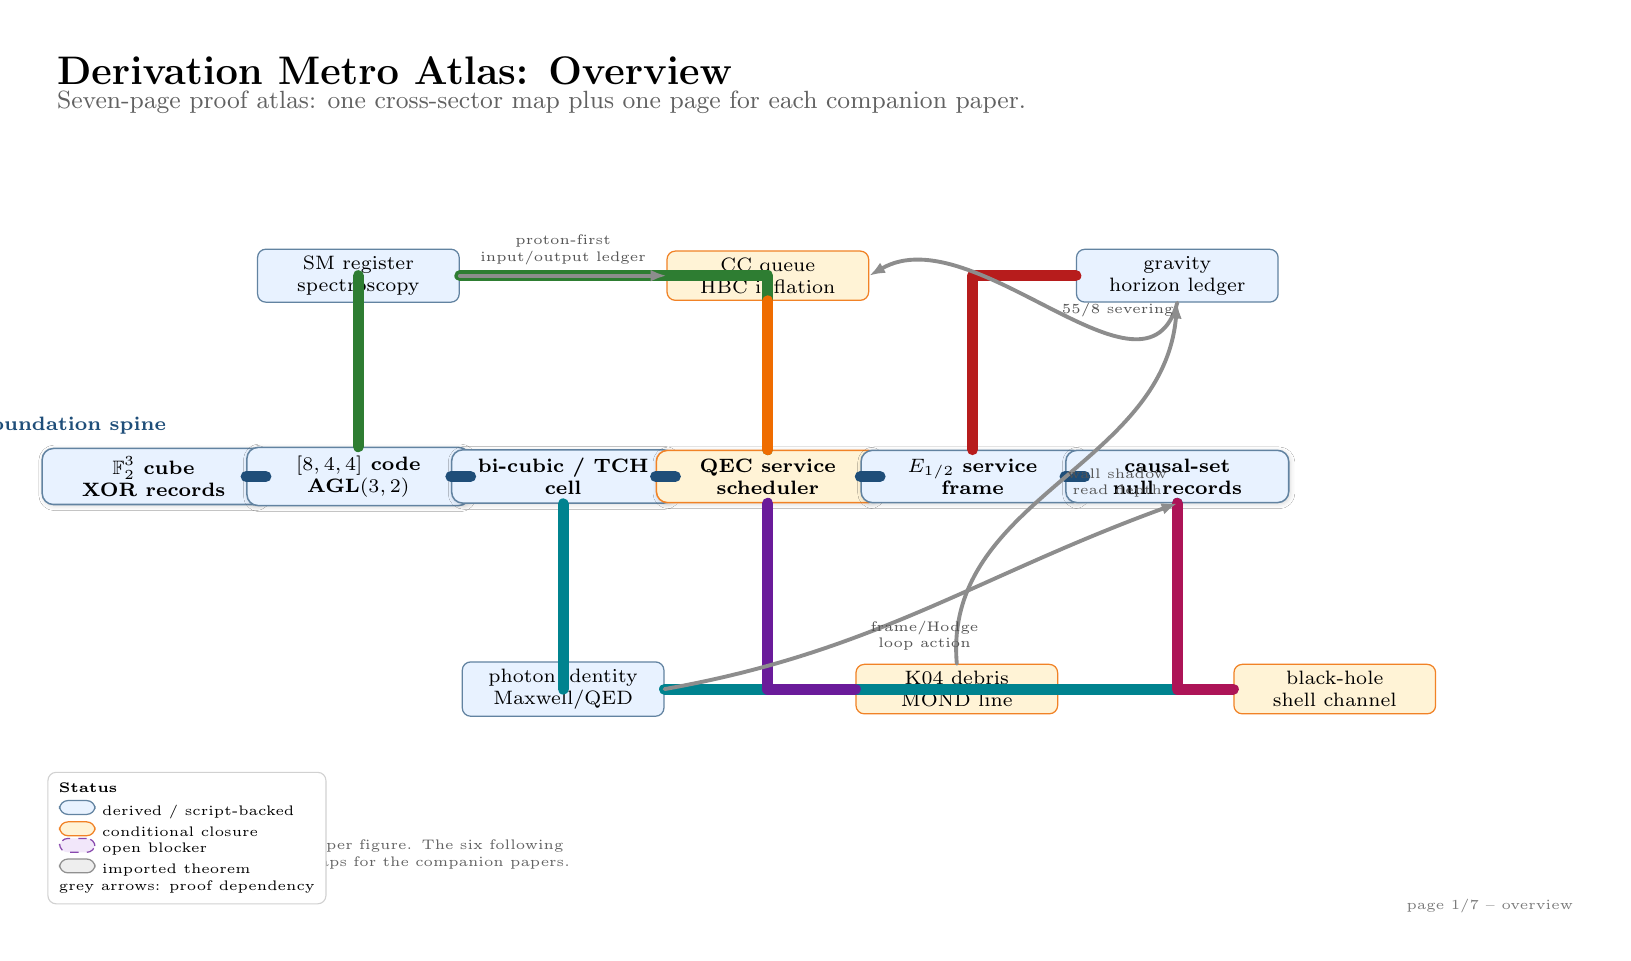
\begin{tikzpicture}[x=1cm,y=1cm]
\pageframe{Derivation Metro Atlas: Overview}
  {Seven-page proof atlas: one cross-sector map plus one page for each companion paper.}
  {page 1/7 -- overview}

\node[hub, derived] (cube) at (1.6,5.8) {$\mathbb F_2^3$ cube\\XOR records};
\node[hub, derived] (code) at (4.2,5.8) {$[8,4,4]$ code\\AGL$(3,2)$};
\node[hub, derived] (cell) at (6.8,5.8) {bi-cubic / TCH\\cell};
\node[hub, conditional] (qec) at (9.4,5.8) {QEC service\\scheduler};
\node[hub, derived] (frame) at (12.0,5.8) {$E_{1/2}$ service\\frame};
\node[hub, derived] (causet) at (14.6,5.8) {causal-set\\null records};
\draw[route, substrate] (cube) -- (code) -- (cell) -- (qec) -- (frame) -- (causet);
\node[routeLabel, text=substrate] at (0.6,6.45) {foundation spine};

\node[station, derived] (matter) at (4.2,8.35) {SM register\\spectroscopy};
\node[station, conditional] (cosm) at (9.4,8.35) {CC queue\\HBC inflation};
\node[station, derived] (grav) at (14.6,8.35) {gravity\\horizon ledger};
\draw[route, matter] (code.north) |- (matter) -| (qec.north);
\draw[route, cosmo] (qec.north) -- (cosm);
\draw[route, gravity] (frame.north) |- (grav);

\node[station, derived] (photon) at (6.8,3.1) {photon identity\\Maxwell/QED};
\node[station, conditional] (darkm) at (11.8,3.1) {K04 debris\\MOND line};
\node[station, conditional] (bh) at (16.6,3.1) {black-hole\\shell channel};
\draw[route, gauge] (cell.south) |- (photon) -| (causet.south);
\draw[route, dark] (qec.south) |- (darkm);
\draw[route, relativity] (causet.south) |- (bh);

\draw[edge] (matter.east) to[out=0,in=180] node[label, above] {proton-first\\input/output ledger} (cosm.west);
\draw[edge] (grav.south) to[out=-105,in=30] node[label, right] {$55/8$ severing} (cosm.east);
\draw[edge] (darkm.north) to[out=95,in=-95] node[label, right] {wall shadow\\read depth} (grav.south);
\draw[edge] (photon.east) to[out=10,in=-160] node[label, below] {frame/Hodge\\loop action} (causet.south);

\node[note, text width=6.7cm] at (3.7,1.0)
  {Use this page as the overview-paper figure. The six following pages are the expanded proof maps for the companion papers.};
\legendblock
\end{tikzpicture}

% ---------------------------------------------------------------------------
% Page 2: foundations and methodology.
% ---------------------------------------------------------------------------
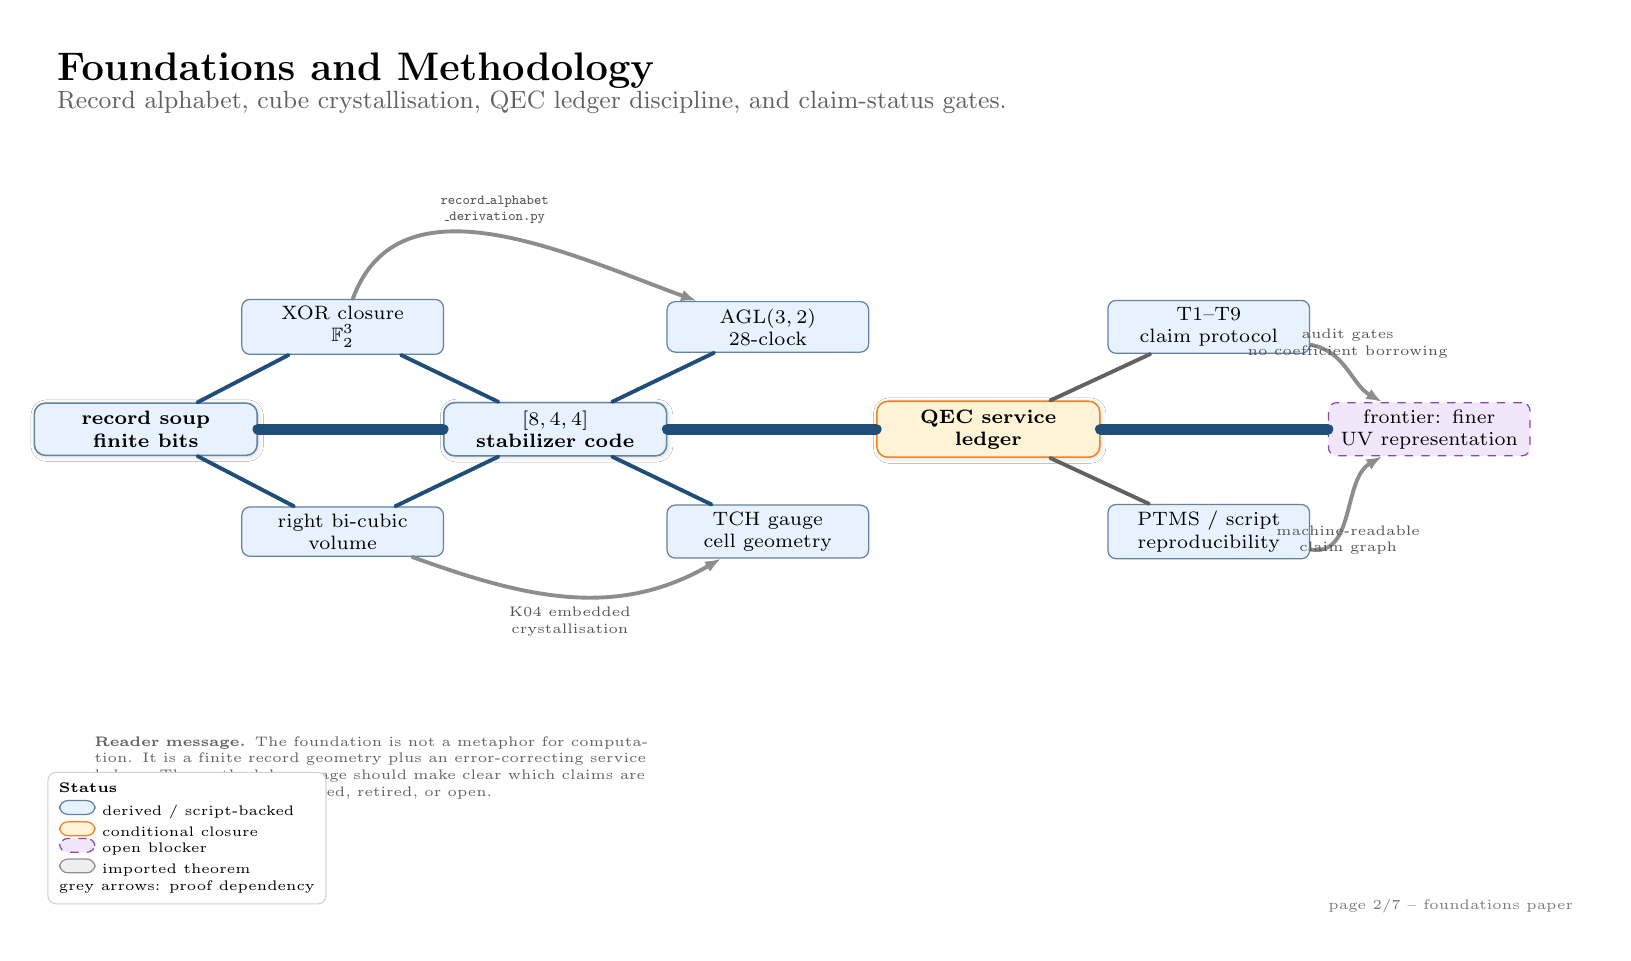
\begin{tikzpicture}[x=1cm,y=1cm]
\pageframe{Foundations and Methodology}
  {Record alphabet, cube crystallisation, QEC ledger discipline, and claim-status gates.}
  {page 2/7 -- foundations paper}

\node[hub, derived] (bits) at (1.5,6.4) {record soup\\finite bits};
\node[station, derived] (xor) at (4.0,7.7) {XOR closure\\$\mathbb F_2^3$};
\node[station, derived] (cube) at (4.0,5.1) {right bi-cubic\\volume};
\node[hub, derived] (code) at (6.7,6.4) {$[8,4,4]$\\stabilizer code};
\node[station, derived] (agl) at (9.4,7.7) {AGL$(3,2)$\\28-clock};
\node[station, derived] (tch) at (9.4,5.1) {TCH gauge\\cell geometry};
\node[hub, conditional] (ledger) at (12.2,6.4) {QEC service\\ledger};
\node[station, derived] (protocol) at (15.0,7.7) {T1--T9\\claim protocol};
\node[station, derived] (ptms) at (15.0,5.1) {PTMS / script\\reproducibility};
\node[station, open] (frontier) at (17.8,6.4) {frontier: finer\\UV representation};

\draw[route, substrate] (bits) -- (code) -- (ledger) -- (frontier);
\draw[soft, substrate] (bits) -- (xor) -- (code);
\draw[soft, substrate] (bits) -- (cube) -- (code);
\draw[soft, substrate] (code) -- (agl);
\draw[soft, substrate] (code) -- (tch);
\draw[soft, method] (ledger) -- (protocol);
\draw[soft, method] (ledger) -- (ptms);

\draw[edge] (xor) to[out=70,in=160] node[label, above] {\texttt{record\_alphabet}\\\texttt{\_derivation.py}} (agl);
\draw[edge] (cube) to[out=-20,in=210] node[label, below] {K04 embedded\\crystallisation} (tch);
\draw[edge] (protocol) to[out=-10,in=150] node[label, above] {audit gates\\no coefficient borrowing} (frontier);
\draw[edge] (ptms) to[out=-10,in=-150] node[label, below] {machine-readable\\claim graph} (frontier);

\node[note, text width=7.3cm] at (4.5,2.1)
  {\textbf{Reader message.} The foundation is not a metaphor for computation. It is a finite record geometry plus an error-correcting service ledger. The methodology page should make clear which claims are derived, conditional, imported, retired, or open.};
\legendblock
\end{tikzpicture}

% ---------------------------------------------------------------------------
% Page 3: matter, gauge structure, and spectroscopy.
% ---------------------------------------------------------------------------
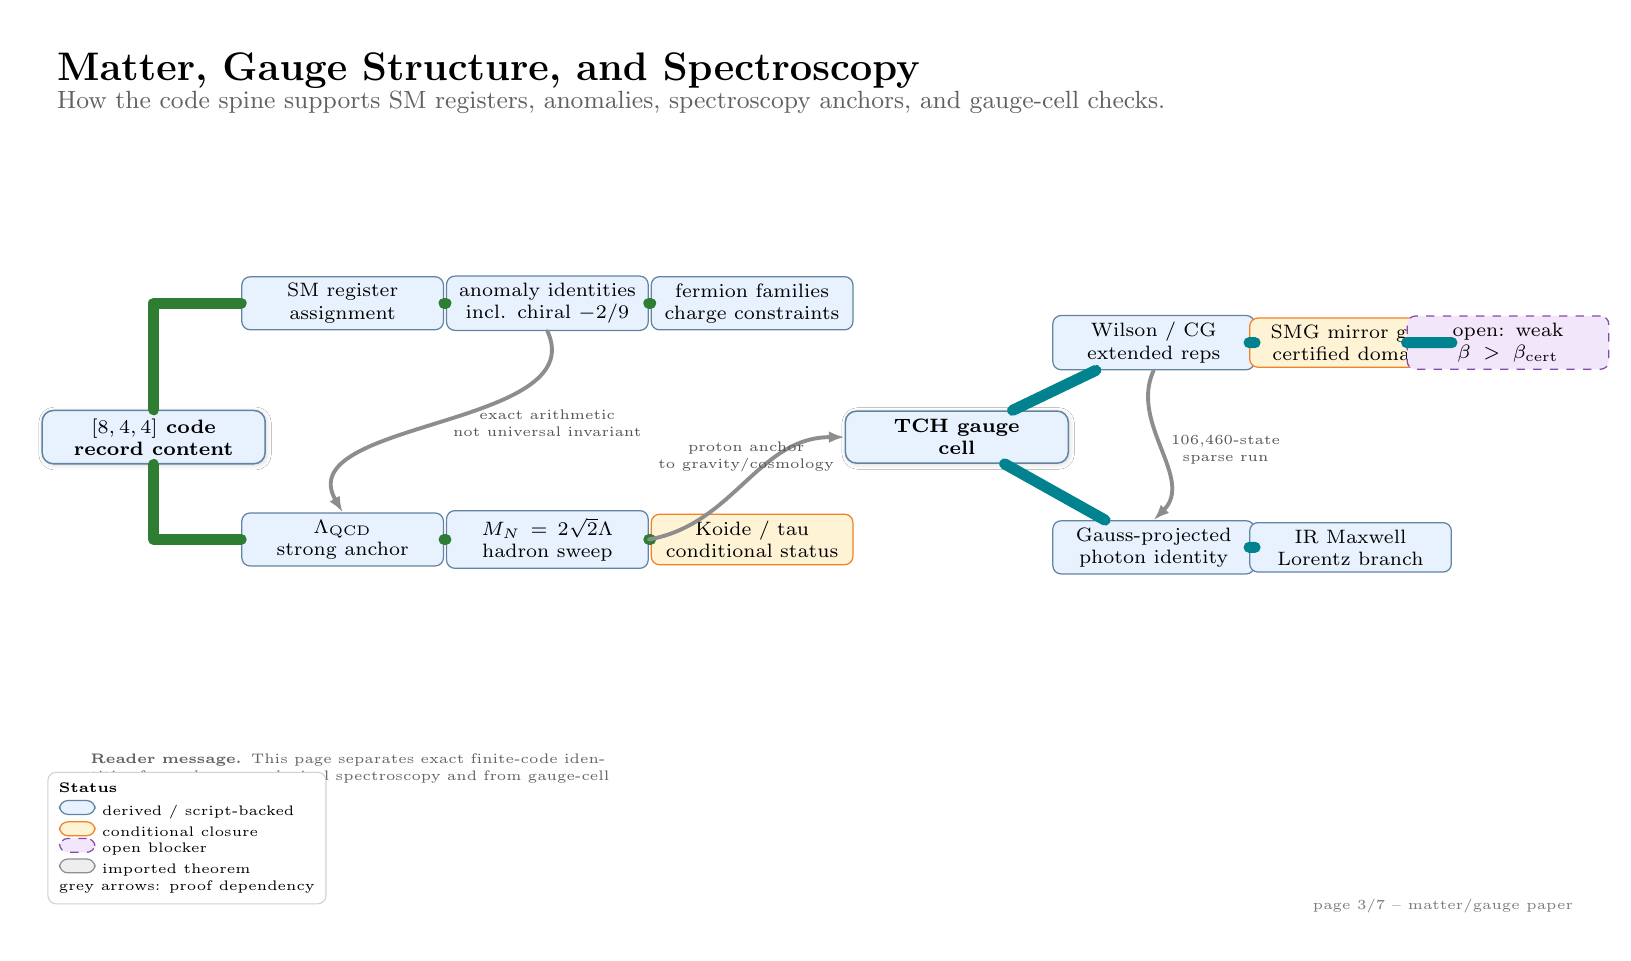
\begin{tikzpicture}[x=1cm,y=1cm]
\pageframe{Matter, Gauge Structure, and Spectroscopy}
  {How the code spine supports SM registers, anomalies, spectroscopy anchors, and gauge-cell checks.}
  {page 3/7 -- matter/gauge paper}

\node[hub, derived] (code) at (1.6,6.3) {$[8,4,4]$ code\\record content};
\node[station, derived] (sm) at (4.0,8.0) {SM register\\assignment};
\node[station, derived] (anom) at (6.6,8.0) {anomaly identities\\incl. chiral $-2/9$};
\node[station, derived] (fermion) at (9.2,8.0) {fermion families\\charge constraints};
\draw[route, matter] (code) |- (sm) -- (anom) -- (fermion);

\node[station, derived] (qcd) at (4.0,5.0) {$\Lambda_{\rm QCD}$\\strong anchor};
\node[station, derived] (hadron) at (6.6,5.0) {$M_N=2\sqrt2\Lambda$\\hadron sweep};
\node[station, conditional] (koide) at (9.2,5.0) {Koide / tau\\conditional status};
\draw[route, matter] (code) |- (qcd) -- (hadron) -- (koide);

\node[hub, derived] (tch) at (11.8,6.3) {TCH gauge\\cell};
\node[station, derived] (wilson) at (14.3,7.5) {Wilson / CG\\extended reps};
\node[station, conditional] (smg) at (16.8,7.5) {SMG mirror gap\\certified domain};
\node[station, open] (beta) at (18.8,7.5) {open: weak\\$\beta>\beta_{\rm cert}$};
\draw[route, gauge] (tch) -- (wilson) -- (smg) -- (beta);

\node[station, derived] (photon) at (14.3,4.9) {Gauss-projected\\photon identity};
\node[station, derived] (ir) at (16.8,4.9) {IR Maxwell\\Lorentz branch};
\draw[route, gauge] (tch) -- (photon) -- (ir);

\draw[edge] (anom.south) to[out=-65,in=120] node[label, right] {exact arithmetic\\not universal invariant} (qcd.north);
\draw[edge] (hadron.east) to[out=10,in=180] node[label, above] {proton anchor\\to gravity/cosmology} (tch.west);
\draw[edge] (wilson.south) to[out=-115,in=45] node[label, right] {106,460-state\\sparse run} (photon.north);

\node[note, text width=6.8cm] at (4.2,2.0)
  {\textbf{Reader message.} This page separates exact finite-code identities from phenomenological spectroscopy and from gauge-cell numerical certification.};
\legendblock
\end{tikzpicture}

% ---------------------------------------------------------------------------
% Page 4: cosmology, dark energy, and inflation.
% ---------------------------------------------------------------------------
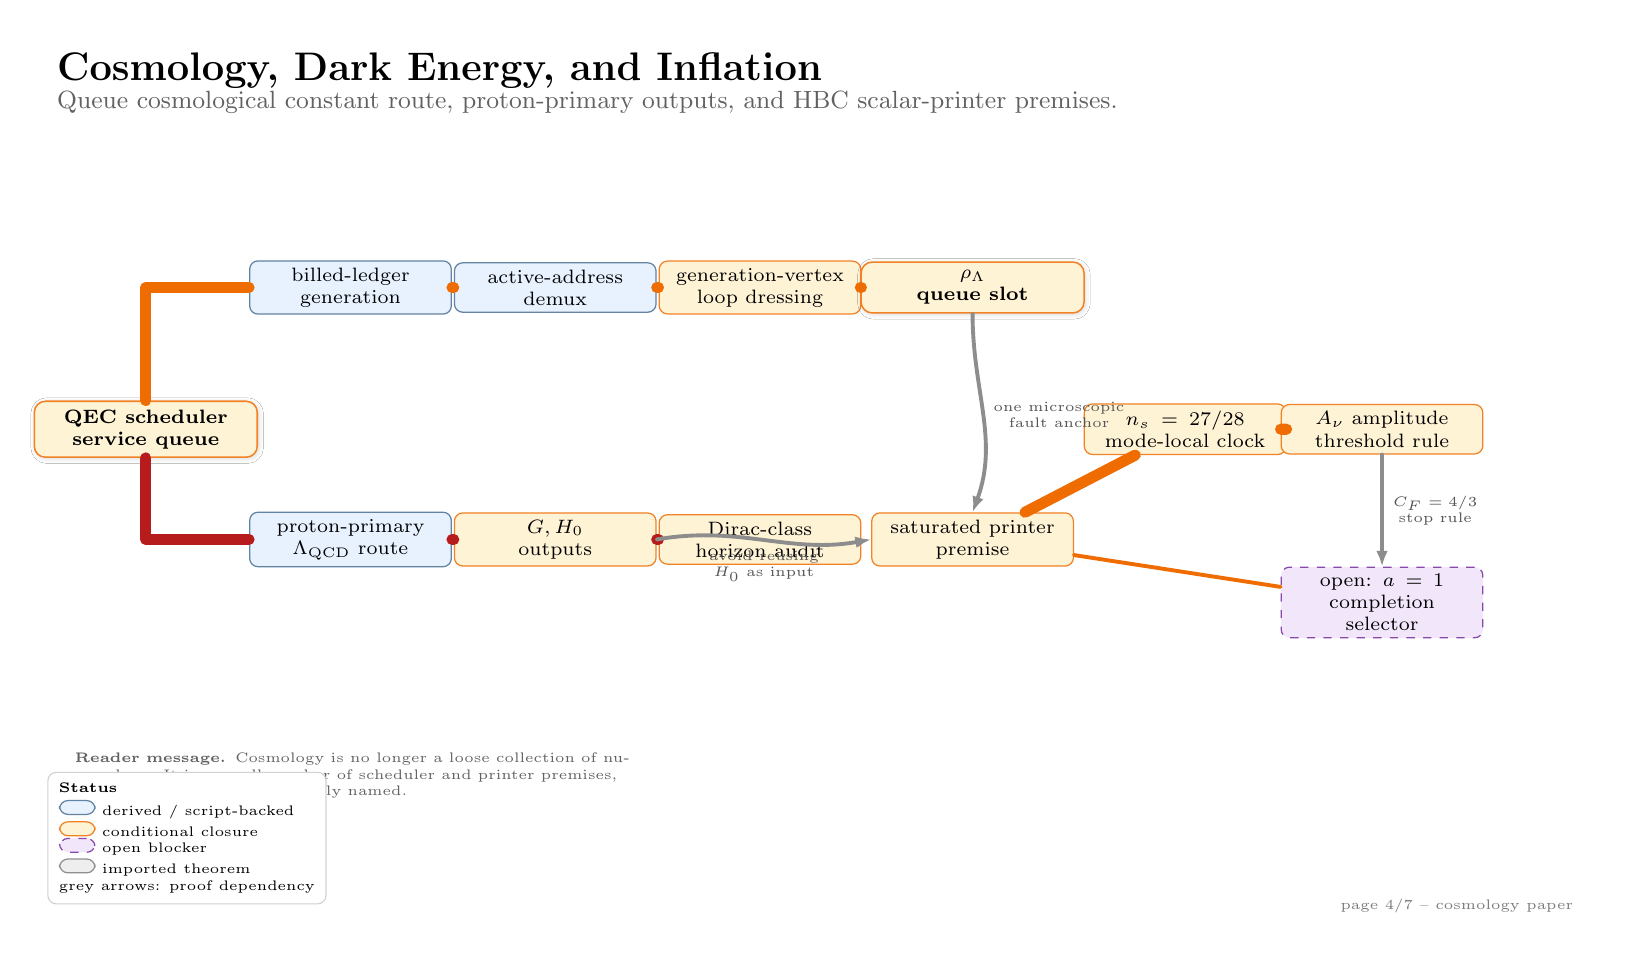
\begin{tikzpicture}[x=1cm,y=1cm]
\pageframe{Cosmology, Dark Energy, and Inflation}
  {Queue cosmological constant route, proton-primary outputs, and HBC scalar-printer premises.}
  {page 4/7 -- cosmology paper}

\node[hub, conditional] (qec) at (1.5,6.4) {QEC scheduler\\service queue};
\node[station, derived] (gen) at (4.1,8.2) {billed-ledger\\generation};
\node[station, derived] (demux) at (6.7,8.2) {active-address\\demux};
\node[station, conditional] (loop) at (9.3,8.2) {generation-vertex\\loop dressing};
\node[hub, conditional] (cc) at (12.0,8.2) {$\rho_\Lambda$\\queue slot};
\draw[route, cosmo] (qec) |- (gen) -- (demux) -- (loop) -- (cc);

\node[station, derived] (proton) at (4.1,5.0) {proton-primary\\$\Lambda_{\rm QCD}$ route};
\node[station, conditional] (gout) at (6.7,5.0) {$G,H_0$\\outputs};
\node[station, conditional] (horizon) at (9.3,5.0) {Dirac-class\\horizon audit};
\draw[route, gravity] (qec) |- (proton) -- (gout) -- (horizon);

\node[station, conditional] (sat) at (12.0,5.0) {saturated printer\\premise};
\node[station, conditional] (tilt) at (14.7,6.4) {$n_s=27/28$\\mode-local clock};
\node[station, conditional] (amp) at (17.2,6.4) {$A_\nu$ amplitude\\threshold rule};
\node[station, open] (completion) at (17.2,4.2) {open: $a=1$\\completion selector};
\draw[route, cosmo] (sat) -- (tilt) -- (amp);
\draw[soft, cosmo] (sat) -- (completion);

\draw[edge] (cc.south) to[out=-90,in=70] node[label, right] {one microscopic\\fault anchor} (sat.north);
\draw[edge] (gout.east) to[out=10,in=190] node[label, below] {avoid reusing\\$H_0$ as input} (sat.west);
\draw[edge] (amp.south) -- node[label, right] {$C_F=4/3$\\stop rule} (completion.north);

\node[note, text width=7.2cm] at (4.2,2.0)
  {\textbf{Reader message.} Cosmology is no longer a loose collection of numerology. It is a small number of scheduler and printer premises, with the live residuals explicitly named.};
\legendblock
\end{tikzpicture}

% ---------------------------------------------------------------------------
% Page 5: dark matter, MOND, and K04 debris.
% ---------------------------------------------------------------------------
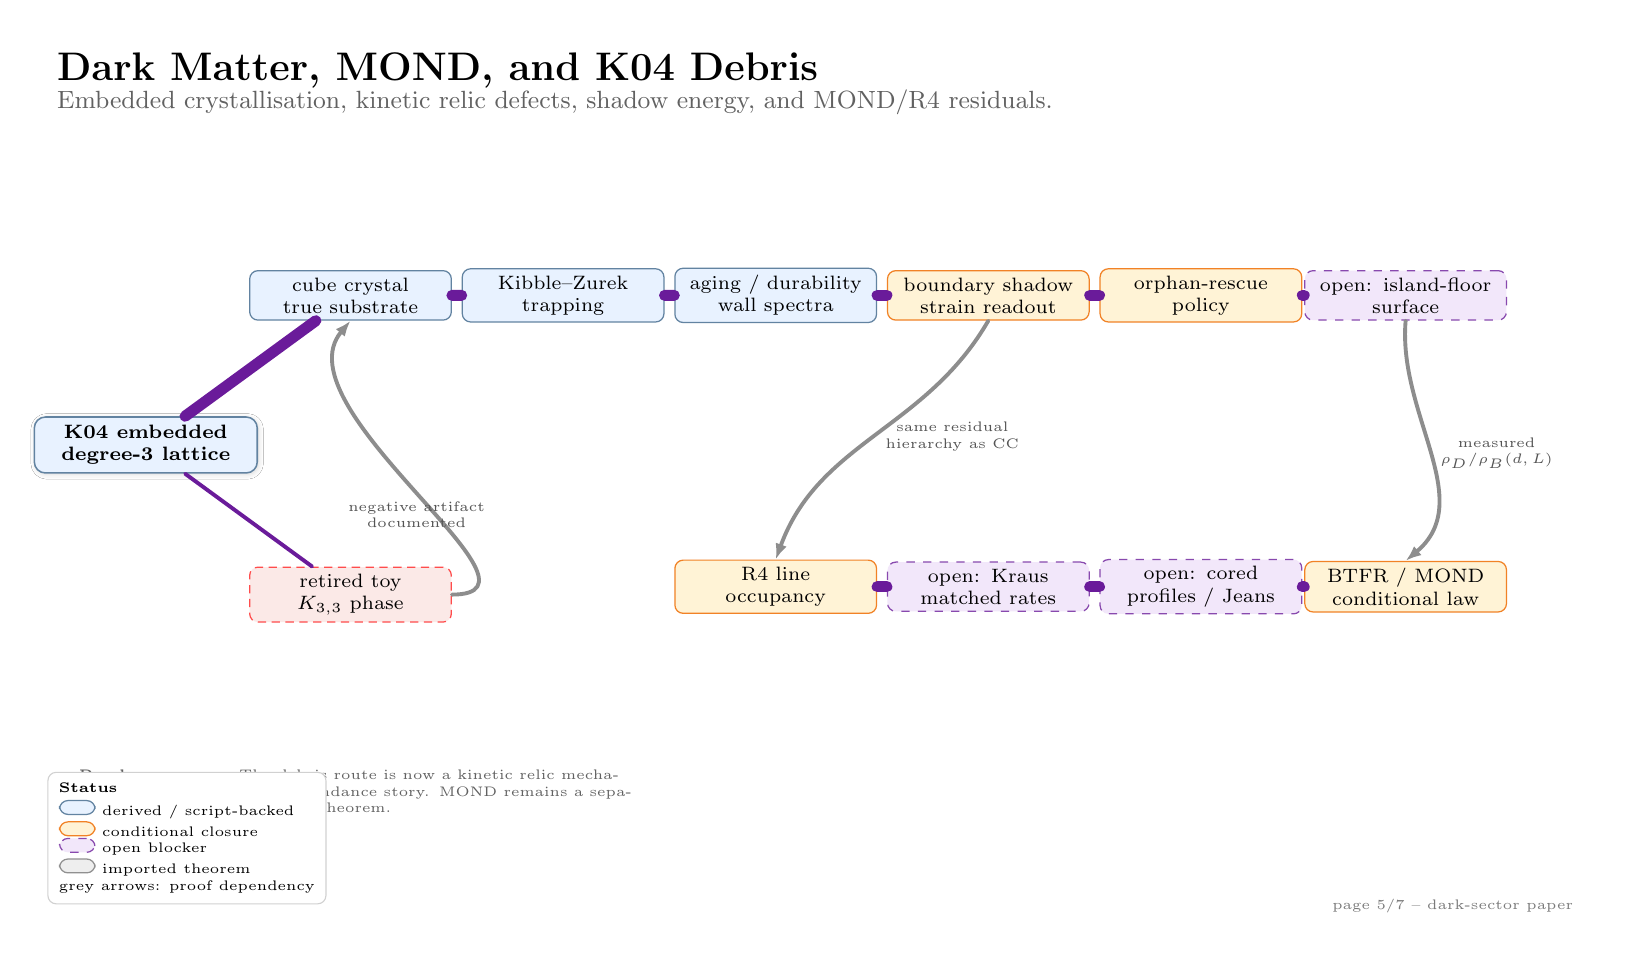
\begin{tikzpicture}[x=1cm,y=1cm]
\pageframe{Dark Matter, MOND, and K04 Debris}
  {Embedded crystallisation, kinetic relic defects, shadow energy, and MOND/R4 residuals.}
  {page 5/7 -- dark-sector paper}

\node[hub, derived] (k04) at (1.5,6.2) {K04 embedded\\degree-3 lattice};
\node[station, derived] (crystal) at (4.1,8.1) {cube crystal\\true substrate};
\node[station, retired] (toy) at (4.1,4.3) {retired toy\\$K_{3,3}$ phase};
\node[station, derived] (kz) at (6.8,8.1) {Kibble--Zurek\\trapping};
\node[station, derived] (aging) at (9.5,8.1) {aging / durability\\wall spectra};
\draw[route, dark] (k04) -- (crystal) -- (kz) -- (aging);
\draw[soft, dark] (k04) -- (toy);

\node[station, conditional] (shadow) at (12.2,8.1) {boundary shadow\\strain readout};
\node[station, conditional] (rescue) at (14.9,8.1) {orphan-rescue\\policy};
\node[station, open] (island) at (17.5,8.1) {open: island-floor\\surface};
\draw[route, dark] (aging) -- (shadow) -- (rescue) -- (island);

\node[station, conditional] (r4) at (9.5,4.4) {R4 line\\occupancy};
\node[station, open] (kraus) at (12.2,4.4) {open: Kraus\\matched rates};
\node[station, open] (profile) at (14.9,4.4) {open: cored\\profiles / Jeans};
\node[station, conditional] (btfr) at (17.5,4.4) {BTFR / MOND\\conditional law};
\draw[route, dark] (r4) -- (kraus) -- (profile) -- (btfr);

\draw[edge] (shadow.south) to[out=-120,in=70] node[label, right] {same residual\\hierarchy as CC} (r4.north);
\draw[edge] (island.south) to[out=-95,in=40] node[label, right] {measured\\$\rho_D/\rho_B(d,L)$} (btfr.north);
\draw[edge] (toy.east) to[out=0,in=-130] node[label, below] {negative artifact\\documented} (crystal.south);

\node[note, text width=7.1cm] at (4.2,1.8)
  {\textbf{Reader message.} The debris route is now a kinetic relic mechanism, not an equilibrium abundance story. MOND remains a separate conditional line-current theorem.};
\legendblock
\end{tikzpicture}

% ---------------------------------------------------------------------------
% Page 6: gravity, horizons, and black holes.
% ---------------------------------------------------------------------------
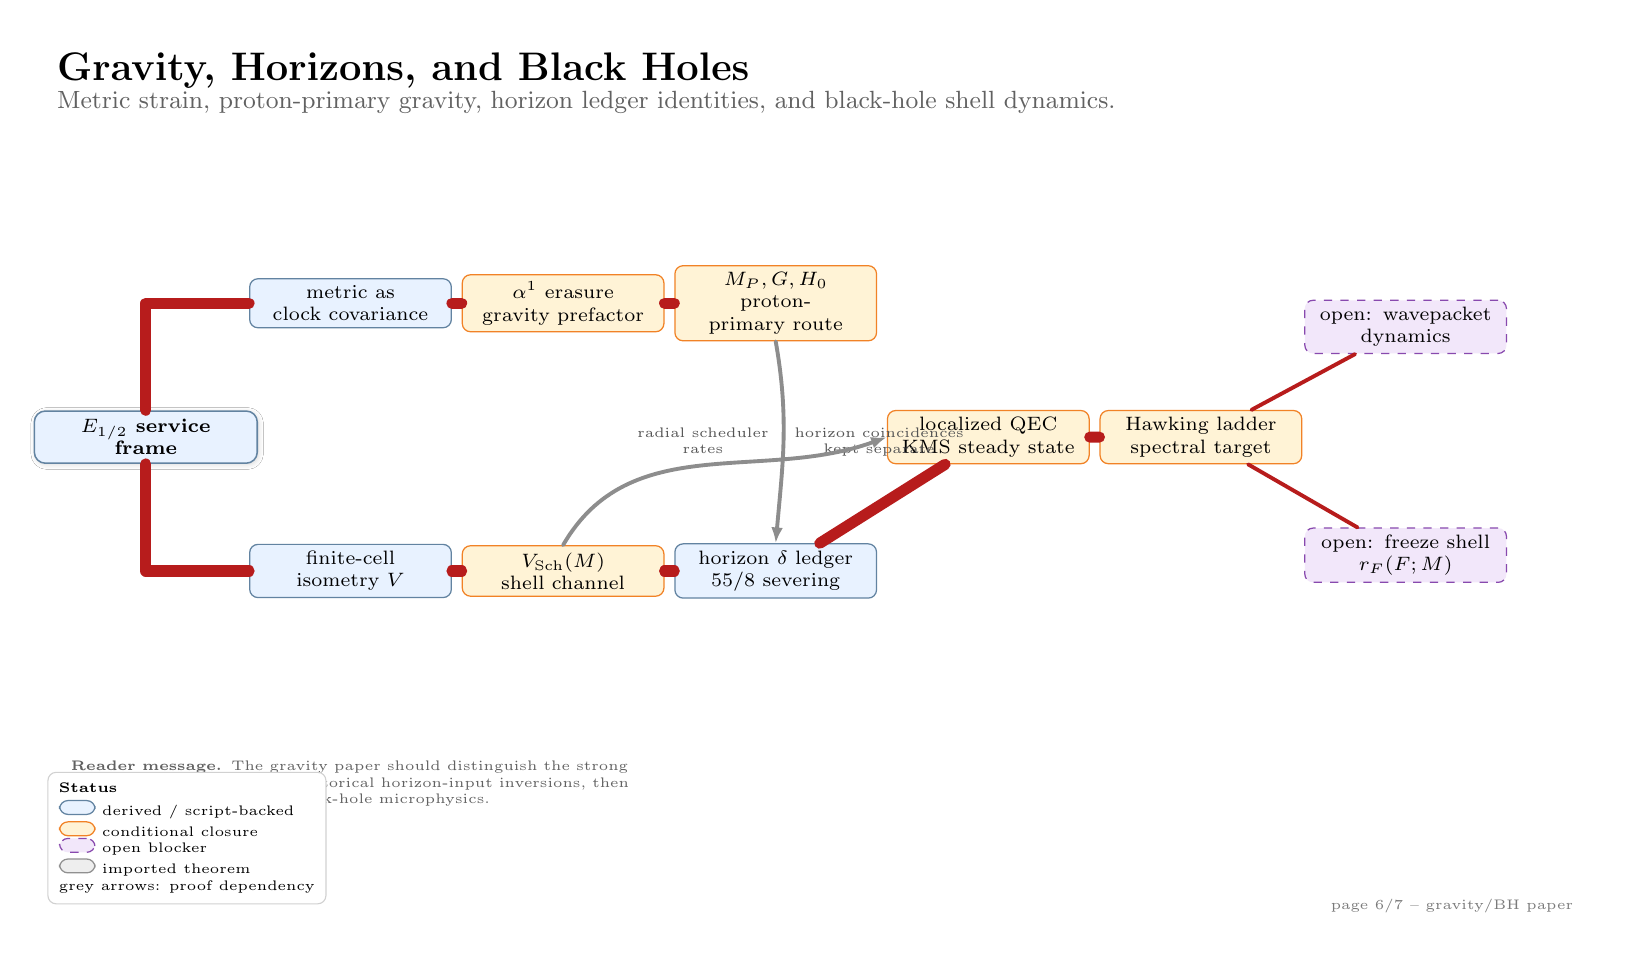
\begin{tikzpicture}[x=1cm,y=1cm]
\pageframe{Gravity, Horizons, and Black Holes}
  {Metric strain, proton-primary gravity, horizon ledger identities, and black-hole shell dynamics.}
  {page 6/7 -- gravity/BH paper}

\node[hub, derived] (frame) at (1.5,6.3) {$E_{1/2}$ service\\frame};
\node[station, derived] (metric) at (4.1,8.0) {metric as\\clock covariance};
\node[station, conditional] (alpha) at (6.8,8.0) {$\alpha^1$ erasure\\gravity prefactor};
\node[station, conditional] (mp) at (9.5,8.0) {$M_P,G,H_0$\\proton-primary route};
\draw[route, gravity] (frame) |- (metric) -- (alpha) -- (mp);

\node[station, derived] (vcell) at (4.1,4.6) {finite-cell\\isometry $V$};
\node[station, conditional] (schw) at (6.8,4.6) {$V_{\rm Sch}(M)$\\shell channel};
\node[station, derived] (delta) at (9.5,4.6) {horizon $\delta$ ledger\\55/8 severing};
\draw[route, gravity] (frame) |- (vcell) -- (schw) -- (delta);

\node[station, conditional] (kms) at (12.2,6.3) {localized QEC\\KMS steady state};
\node[station, conditional] (hawking) at (14.9,6.3) {Hawking ladder\\spectral target};
\node[station, open] (wave) at (17.5,7.7) {open: wavepacket\\dynamics};
\node[station, open] (freeze) at (17.5,4.8) {open: freeze shell\\$r_F(F;M)$};
\draw[route, gravity] (delta) -- (kms) -- (hawking);
\draw[soft, gravity] (hawking) -- (wave);
\draw[soft, gravity] (hawking) -- (freeze);

\draw[edge] (mp.south) to[out=-80,in=85] node[label, right] {horizon coincidences\\kept separate} (delta.north);
\draw[edge] (schw.north) to[out=60,in=200] node[label, above] {radial scheduler\\rates} (kms.west);

\node[note, text width=7.3cm] at (4.2,1.9)
  {\textbf{Reader message.} The gravity paper should distinguish the strong proton-primary route from historical horizon-input inversions, then use the horizon ledger for black-hole microphysics.};
\legendblock
\end{tikzpicture}

% ---------------------------------------------------------------------------
% Page 7: relativity, photon, and causal-set QED.
% ---------------------------------------------------------------------------
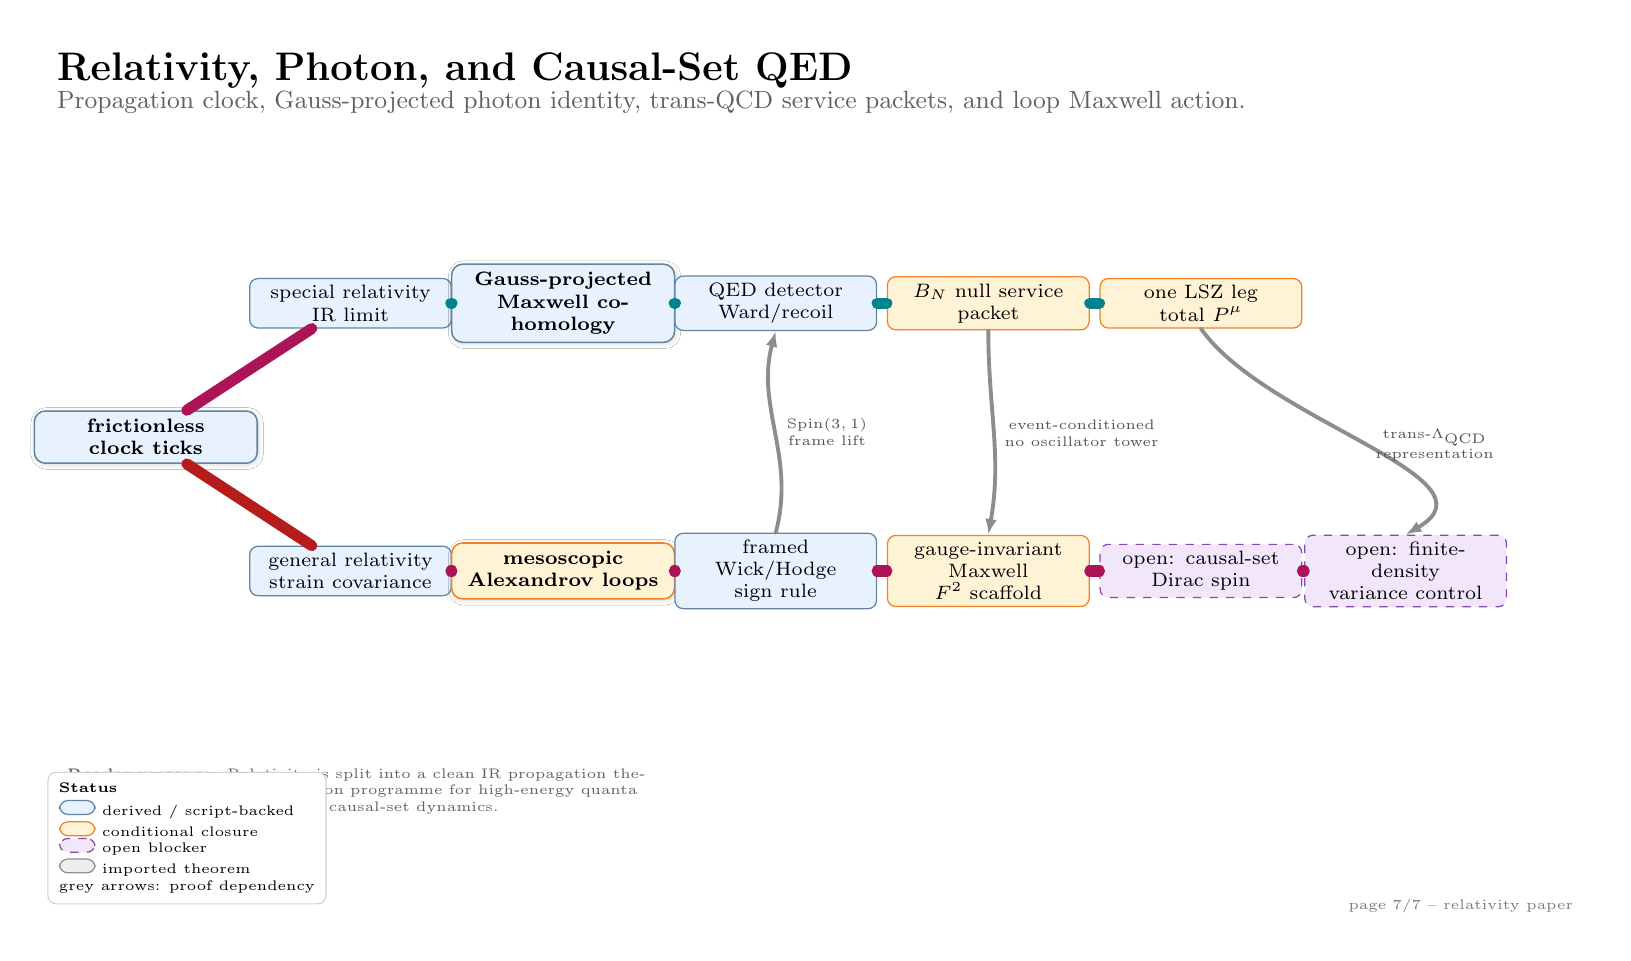
\begin{tikzpicture}[x=1cm,y=1cm]
\pageframe{Relativity, Photon, and Causal-Set QED}
  {Propagation clock, Gauss-projected photon identity, trans-QCD service packets, and loop Maxwell action.}
  {page 7/7 -- relativity paper}

\node[hub, derived] (clock) at (1.5,6.3) {frictionless\\clock ticks};
\node[station, derived] (sr) at (4.1,8.0) {special relativity\\IR limit};
\node[station, derived] (gr) at (4.1,4.6) {general relativity\\strain covariance};
\draw[route, relativity] (clock) -- (sr);
\draw[route, gravity] (clock) -- (gr);

\node[hub, derived] (gauss) at (6.8,8.0) {Gauss-projected\\Maxwell cohomology};
\node[station, derived] (ward) at (9.5,8.0) {QED detector\\Ward/recoil};
\node[station, conditional] (bn) at (12.2,8.0) {$B_N$ null service\\packet};
\node[station, conditional] (lsz) at (14.9,8.0) {one LSZ leg\\total $P^\mu$};
\draw[route, gauge] (sr) -- (gauss) -- (ward) -- (bn) -- (lsz);

\node[hub, conditional] (loops) at (6.8,4.6) {mesoscopic\\Alexandrov loops};
\node[station, derived] (hodge) at (9.5,4.6) {framed Wick/Hodge\\sign rule};
\node[station, conditional] (f2) at (12.2,4.6) {gauge-invariant\\Maxwell $F^2$ scaffold};
\node[station, open] (dirac) at (14.9,4.6) {open: causal-set\\Dirac spin};
\node[station, open] (variance) at (17.5,4.6) {open: finite-density\\variance control};
\draw[route, relativity] (gr) -- (loops) -- (hodge) -- (f2) -- (dirac) -- (variance);

\draw[edge] (bn.south) to[out=-90,in=80] node[label, right] {event-conditioned\\no oscillator tower} (f2.north);
\draw[edge] (hodge.north) to[out=75,in=-105] node[label, right] {Spin$(3,1)$\\frame lift} (ward.south);
\draw[edge] (lsz.south) to[out=-55,in=30] node[label, right] {trans-$\Lambda_{\rm QCD}$\\representation} (variance.north);

\node[note, text width=7.4cm] at (4.2,1.8)
  {\textbf{Reader message.} Relativity is split into a clean IR propagation theorem and a harder representation programme for high-energy quanta and manifestly gauge-invariant causal-set dynamics.};
\legendblock
\end{tikzpicture}

\end{document}
